

\chapter{外文资料原文}
\label{cha:engorg}

\title{Unsupervised 3D registration through optimization-guided cyclical self-training}

\textbf{Abstract:}State-of-the-art deep learning-based registration methods employ three different learning strategies: supervised learning, which requires costly manual annotations, unsupervised learning, which heavily relies on hand-crafted similarity metrics designed by domain experts, or learning from synthetic data, which introduces a domain shift. To overcome the limitations of these strategies, we propose a novel selfsupervised learning paradigm for unsupervised registration, relying on self-training. Our idea is based on two key insights. Feature-based differentiable optimizers 1) perform reasonable registration even from random features and 2) stabilize the training of the preceding feature extraction network on noisy labels. Consequently, we propose cyclical self-training, where pseudo labels are initialized as the displacement fields inferred from random features and cyclically updated based on more and more expressive features from the learning feature extractor, yielding a selfreinforcement effect. We evaluate the method for abdomen and lung registration, consistently surpassing metric-based supervision and outperforming diverse state-of-the-art competitors. Source code is available at https://github.com/multimodallearning/reg-cyclical-self-train.

\section{Introduction}

Medical image registration is a fundamental task in medical imaging with applications ranging from multi-modal data fusion to temporal data analysis. In recent years, deep learning has advanced learning-based registration methods [11], which achieve competitive performances at low runtimes and thus constitute a promising alternative to accurate but slow classical optimization methods. A decisive factor in successfully training deep learning-based methods is the choice of a suitable strategy to supervise the learning process. In the literature, there exist three different learning strategies. The first is supervised learning based on manual annotations such as landmark correspondences [9] or semantic labels [16]. However, manual annotations are costly and may introduce a label bias [2]. Alternatively, a second strategy employs synthetic deformation fields to generate image pairs with precisely known displacement fields [7]. However, this introduces a domain gap between synthetic training and real test pairs, limiting the performance at inference time. Elaborated deformation techniques can reduce the gap but require strong domain knowledge, are tailored to specific problems, and do not generalize across tasks. The third widely used training strategy is unsupervised metric-based learning, maximizing a similarity metric between fixed and warped moving images, e.g. implemented in [2,17]. Popular metrics include normalized cross-correlation [19] and MIND [13]. However, the success of this strategy strongly depends on the specific hand-crafted metric, and the performance of the trained deep learning models is often inferior to a classical optimization-based counterpart. Considering the deficiencies of the above training techniques, in this work, we introduce a novel learning strategy for unsupervised registration based on the concept of self-training. Self-training is a widespread training strategy for semi-supervised learning [24] and domain adaptation [29]. The core idea is to pre-train a network on available labeled data and subsequently apply the model to the unlabeled data to generate so-called pseudo labels. Afterwards, one alternates between re-training the model on the union of labeled and pseudo-labeled data and updating the pseudo labels with the current model. This general concept was successfully adapted to diverse tasks and settings, with methods in medical context primarily focusing on segmentation [8,18]. These methods resort to a special form of self-training, the Mean Teacher paradigm [22], where pseudo labels are continuously provided by a teacher model, representing a temporal ensemble of the learning network. A persistent problem of classical and Mean Teacher-based selftraining is the inherent noise of the pseudo labels, which can severely hamper the learning process. As a remedy, some works aim to filter reliable pseudo labels based on model uncertainty [28]. Only recently, the Mean Teacher was adapted to the registration problem, tackling domain adaptation [3] or complementing metric-based supervision for adaptive regularization weighting [25]. Contrary to these methods, we introduce self-training for registration in a fully unsupervised setting, with pseudo labels as the single source of supervision.

\textbf{Contributions.}

We introduce a novel learning paradigm for unsupervised registration by adapting the concept of self-training to the problem. This involves two principal challenges. First, labeled data for the pre-training stage is unavailable, raising the question of how to generate initial pseudo labels. Second, as a general problem in self-training, the negative impact of noise in the pseudo labels needs to be mitigated. In our pursuit to overcome these challenges, we made two decisive observations (see Fig.2) when exploring a combination of deep learning-based feature extraction with differentiable optimization algorithms for the displacement prediction, such as [9,20]. First, we found that feature-based optimizers predict reasonable displacement fields and improve the initial registration even when applied to the output of random feature networks (orange line in Fig.2). We attribute this feature to the inductive bias of deep neural networks, which extract somewhat useful features even with random weights [4]. These predicted displacements thus constitute meaningful initial pseudo labels, solving the first problem and leaving us with the second problem to overcome the noise in the labels. In this context, we made the second observation that the intrinsic regularizing capacity of the optimizers stabilizes the learning from noisy labels. Specifically, training the feature extractor on our initial pseudo labels yielded registrations surpassing the accuracy of the noisy labels used for training (green, red, purple, brown, and magenta lines in Fig.2). Consequently, we propose a cyclical self-training scheme, alternating between training the feature extractor and updating the pseudo labels. As such, our novel learning paradigm does not require costly manual annotations, prevents the domain shift of synthetic deformations, and is independent of hand-crafted similarity metrics. Moreover, our method significantly differs from previous uncertainty-based pseudo label filtering strategies since it implicitly overcomes the negative impact of noisy labels by combining deep feature learning with regularizing differentiable optimization. We evaluate the method for CT abdomen registration and keypoint-based lung registration, demonstrating substantial improvements over diverse state-of-theart comparison methods.

\section{Methods}

\subsection{Problem setup}

Given a data pair ($F$,$M$) of a fixed and a moving image as input, registration aims at finding a displacement field $\varphi$ that spatially aligns $M$ to $F$ . We address the task in an unsupervised setting, where training data $\mathcal{T}=\{(\boldsymbol{F}_i,\boldsymbol{M}_i)\}_{i=1}^{|\mathcal{T}|}$  consists of $|\mathcal{T}|$ unlabeled data pairs. Given the training data, we aim to learn a function $f$ with parameters $\theta_f$ , (partially) represented by a deep network, which predicts displacement fields as $ \hat{\boldsymbol{\varphi}}=f(\boldsymbol{F},\boldsymbol{M};\boldsymbol{\theta}_f)$.

\subsection{Cyclical self-training}

We propose to solve the above problem with a cyclical self-training strategy visualized in Fig.1. While existing self-training methods assume the availability of some labeled data, annotations are unavailable in our unsupervised setting. To overcome this issue and generate an initial set of pseudo labels for the first stage of self-training, we parameterize the function $f$ as the combination of a deep neural network $g$ for feature extraction with a non-learnable but differentiable feature-based optimization algorithm $h$ for displacement prediction, i.e.

\begin{figure}
  \centering
  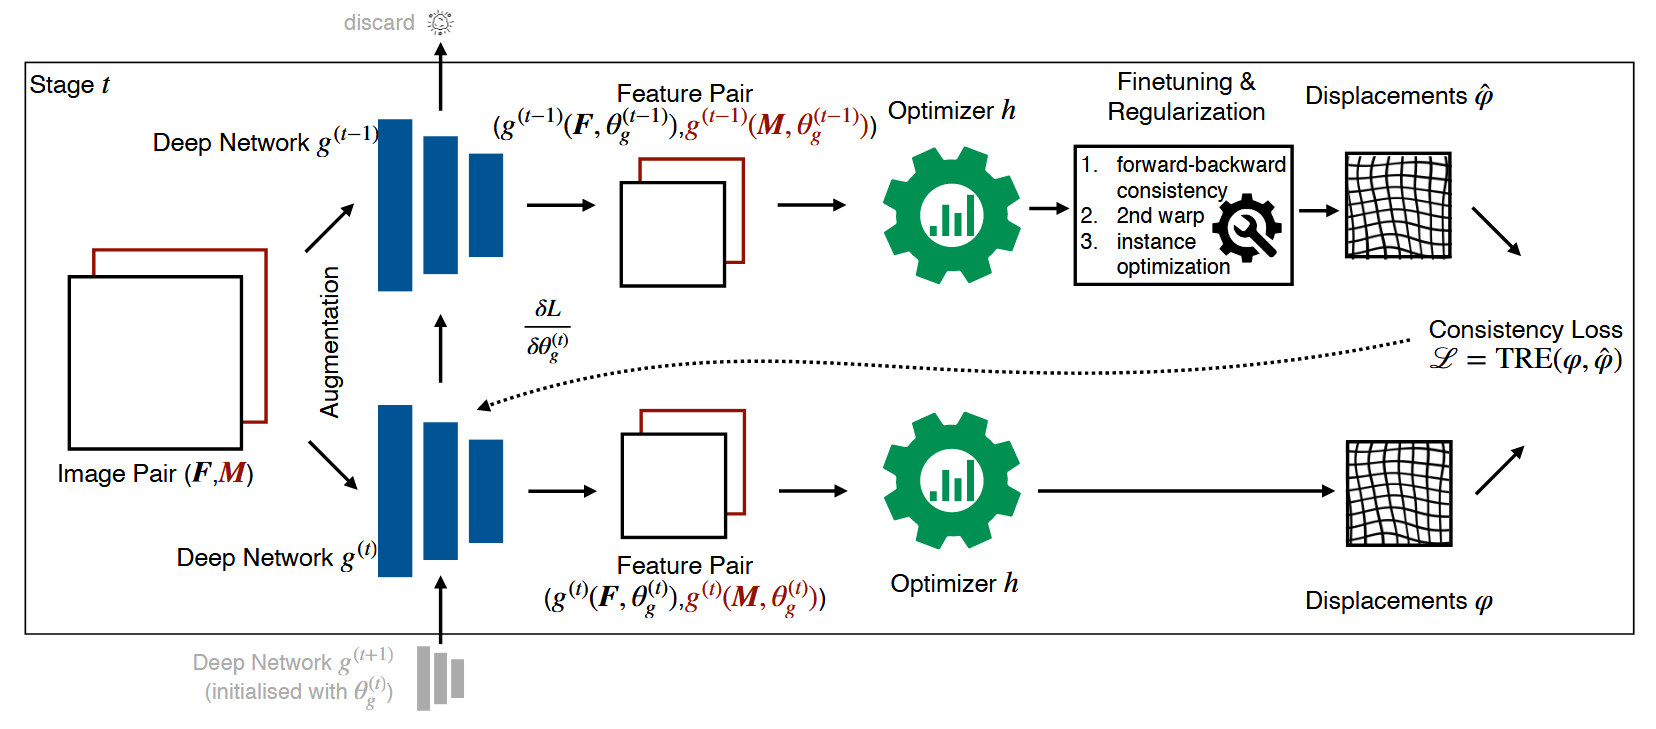
\includegraphics[width=0.9\textwidth]{T_RegCST.png}
  \bicaption[t-fig:1]{无监督注册的循环自训练范式概述}{底层配准流水线包括用于特征提取的深度网络g和用于预测位移的可微优化器h。在阶段t,我们使用基于前一阶段网络g(t-1)的特征生成的伪标签来监督网络g(t)的训练。对于最优特征学习,优化器的伪位移被进一步细化和正则化。}{Fig.$\!$ }{Overview of the proposed cyclical self-training paradigm for unsupervised registration. The underlying registration pipeline comprises a deep network for feature extraction g and a differentiable optimizer h to predict the displacements. At stage t, we supervise the training of the network $g^{(t)}$ with pseudo labels generated based on the features from the network $g^{(t-1)}$ from the previous stage. For optimal feature learning, the pseudo displacements from the optimizer are further refined and regularized.}
\end{figure}

\begin{equation}\tag*{(1)}
  f(\boldsymbol{F},\boldsymbol{M};\boldsymbol{\theta}_f)=h(g(\boldsymbol{F},\boldsymbol{M};\boldsymbol{\theta}_g))
\end{equation}

The approach is based on our empirical observation that a suitable optimization algorithm $h$ can predict reasonable initial displacement fields $\hat{\boldsymbol{\varphi}}^{(0)}$ from random features provided by a network $g^{(0)}$ with random initialization$\theta_G^{(0)} $, which is in line with recent studies on the inductive bias of CNNs [4]. We leverage these predicted displacements as pseudo labels to supervise the first stage of self-training,where the parameters of the feature extractor with different initialization$\theta_G^{(1)} $are optimized by minimizing the loss

\begin{equation}\tag*{(2)}
  \mathcal{L}(\boldsymbol{\theta}_g^{(1)};\mathcal{T})=\frac{1}{|\mathcal{T}|}\sum_i\mathrm{TRE}\left(h\left(g\left(\boldsymbol{F}_i,\boldsymbol{M}_i;\boldsymbol{\theta}_g^{(1)}\right)\right),\hat{\boldsymbol{\varphi}}_i^{(0)}\right)
\end{equation}

with $\mathrm{TRE}(\hat{\boldsymbol{\varphi}}_\mathrm{i}^{(1)},\hat{\boldsymbol{\varphi}}_\mathrm{i}^{(0)})$ denoting the mean over the element-wise target registration error between the displacement fields $\hat{\boldsymbol{\varphi}}_\mathrm{i}^{(1)} $ and $\hat{\boldsymbol{\varphi}}_\mathrm{i}^{(0)}$.

A critical problem of this basic setup is that the network might overfit the initial pseudo labels and learn to reproduce random features. Therefore, in the spirit of recent techniques from contrastive learning [6], we propose to improve the efficacy of feature learning by incorporating asymmetries into the learning and pseudo label streams at two levels. First, we apply different random augmentations to the input pairs in both streams. Second, we augment the pseudo label stream with additional (non-differentiable) fine-tuning and regularization steps after the optimizer to improve the pseudo displacement fields (see Sec. 2.3 for details). As demonstrated in our ablation experiments (Fig.2, Tab.1), both strategies improve feature learning and strengthen the self-improvement effect.

Once the first stage of self-training has converged, we repeat the process $T$ times. Specifically, at stage $t$, we generate refined pseudo labels with the trained network $g^{(t-1)}$ from the previous stage, initialize the learning network $g^{(t)}$ with the weights from $g^{(t-1)}$ and perform a warm restart on the learning rate to escape potential local minima from the previous stage.

\subsection{Registration framework}

Our proposed self-training scheme is a flexible, modular framework, agnostic to the input modality and the specific implementation of feature extractor $g$ and optimizer $h$. This section describes our specific design choices for $g$ and $h$ for image and point cloud registration, with the former being our main focus.


\textbf{Image registration.} To extract features from 3D input volumes, we implement g a standard 3D CNN with six convolution layers with kernel sizes 3 $\times$ 3 $\times$ 3 and 32, 64, or 128 channels. Each convolution is followed by BatchNorm and ReLU, and every second convolution contains a stride of 2, yielding a downsampling factor of 8. The outputs for both images are mapped to 16-dimensional features using a 1 $\times$ 1 $\times$ 1 convolution and fed into a correlation layer [21] that captures 125 discrete displacements.

As the optimizer, we adapt the coupled convex optimization for learningbased 3D registration from [20], which, given fixed and moving features, infers a displacement field that minimizes a combined objective of smoothness and feature dissimilarity. Our proposed refinement strategy in the pseudo label stream comprises three ingredients. 1) Forward-backward consistency additionally computes the reverse displacement field ($\boldsymbol{F}$ to $\boldsymbol{M}$ ) and then iteratively minimizes the discrepancy between both fields. 2) For a second warp, the moving image is warped with the inferred displacement field before repeating all previous steps. 3) Iterative instance optimization finetunes the final displacement field with Adam by jointly minimizing regularization cost and feature dissimilarity. For the latter, we use the CNN features after the second convolution block and map them with a 1$\times$1$\times$1 convolution to 16 channels. We apply the same refinement steps at test time. Moreover, we propose to leverage the difference between network-predicted and finetuned displacements to estimate the difficulty of the training samples. Consequently, we apply a weighted batch sampling at training that increases the probability of using less difficult registration pairs with a higher agreement between both fields. We rank all training pairs and use a sigmoid function with arguments ranging linearly from -5 to 5 for the weighted random sampler.

\textbf{Point cloud registration.} For point cloud registration, we implement the feature extractor as a graph CNN and rely on sparse loopy belief propagation for differentiable optimization, as introduced in [9].

\section{Experiments}

\subsection{Experimental setup}

\textbf{Datasets.} We conduct our main experiments for inter-patient abdomen CT registration using the corresponding dataset of the Learn2Reg (L2R) Challenge [15]. The dataset contains 30 abdominal 3D CT scans of different patients with 13 manually labeled anatomical structures of strongly varying sizes. The original image data and labels are from [26]. As part of L2R, they were affinely preregistered into a canonical space and resampled to identical voxel resolutions (2 mm) and spatial dimensions (192 $\times$ 160 $\times$ 256 vx). Following the data split of L2R, we use 20 scans (190 pairs) for training and the remaining 10 scans (45 pairs) for evaluation. Hence, data split and preprocessing are consistent with compared previous works [9,27]. As metrics, we report the mean Dice overlap (DSC) between the semantic labels and the standard deviation of the logarithmic Jacobian determinant (SDlogJ).

We perform a second experiment for inhale-to-exhale lung CT registration on the DIR-Lab COPDGene dataset5 [5], which comprises 10 such scan pairs. For each pair, 300 expert-annotated landmark correspondences are available for evaluation. We pre-process all scans in multiple steps: 1) resampling to 1.75$\times$1.00$\times$1.25 mm for exhale and 1.75$\times$1.25$\times$1.75 mm for inhale, 2) cropping with fixed-size bounding boxes (192 $\times$ 192 $\times$ 208 vx), centered around automatically generated lung masks, 3) affine pre-registration, aligning the lung masks. Since we focus on keypoint-based registration of the lung CTs, we follow [9] and extract distinctive keypoints from the CTs using the Förstner algorithm with non-maximum suppression, yielding around 1k points in the fixed and 2k points in the moving cloud. In our experiments, we perform 5-fold cross-validation, with each fold comprising eight data pairs for training and two for testing. We report the target registration error (TRE) at the landmarks and the SDlogJ as metrics.

\textbf{Implementation details.} We implement all methods in Pytorch and optimize network parameters with the Adam optimizer. For abdomen registration, we train for $T$ = 8 stages, each stage comprising 1000 iterations with a batch size of 2. The learning rate follows a cosine annealing warm restart schedule, decaying from $10^{-3}$ to $10^{-5}$ at each stage. Hyper-parameters were set based on the DSC on three cases from the training set. For lung registration, the model converged after $T$ = 5 stages of 60 epochs with batch size 4, with an initial learning rate of 0.001, decreased by a factor of 10 at epochs 40 and 52. Here, hyper-parameters were adopted from [9]. For both datasets, training requires 90-100 min and 8 GB on an RTX2080, and input augmentations consist of random affine transformations.

\subsection{Results}

\textbf{Abdomen. }First, we analyze our method in several ablation experiments. In Fig.2, we visualize the performance of our method on a subset of classes over several cycles of self-training. We observe consistent improvements over the stages, particularly pronounced at early stages while the performance converges later on. This highlights the self-reinforcing effect achieved through alternating pseudo label updates and network training. In the upper part of Tab.1, we verify the efficacy of incorporating asymmetries (input augmentations, finetuning of pseudo labels) into both streams and weighted sampling. The results confirm the importance of each component to reach optimal performance. In the lower part of Tab.1, we evaluate our final model under different test configurations, highlighting the improvements through a second warp and Adam finetuning.

\begin{figure}
  \centering
  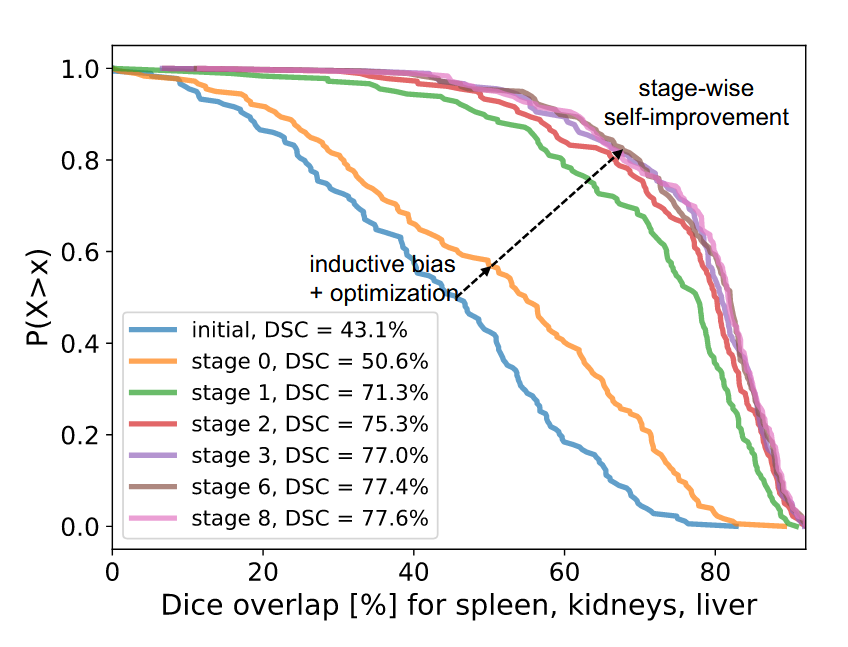
\includegraphics[width=0.9\textwidth]{T_result.png}
  \bicaption[t-fig:2]{}{在不同阶段的自我训练后,腹部CT登记的Dice重叠的“相反”累积分布。}{Fig.$\!$ }{“Opposite” cumulative distribution of Dice overlaps for Abdomen CT registration after different stages of self-training.}
\end{figure}

\begin{table}
  \bicaption[t:table1]{}{腹部CT配准的消融研究。}{Table$\!$}{Ablation study for abdomen CT registration.}
  \vspace{0.5em}\centering\wuhao
  \begin{tabular}{lcc}
    \toprule
    \textbf{Method}       & \textbf{DSC}  & \textbf{SDlogJ} \\
    \midrule
    prealign              & 25.9          & --              \\
    w/o input augm.       & 48.8          & 0.129           \\
    w/o PL refinement     & 48.8          & 0.200           \\
    w/o weighted sampling & 50.1          & 0.147           \\
    ours                  & 51.1          & 0.146           \\
    \midrule
    1 warp w/o Adam       & 38.6          & 0.061           \\
    1 warp w/ Adam        & 49.6          & 0.119           \\
    2 warps w/o Adam      & 41.1          & 0.088           \\
    2 warps w/Adam (ours) & \textbf{51.1} & 0.146           \\
    \bottomrule
  \end{tabular}
\end{table}

Next, we compare our method to a comprehensive set of state-of-the-art unsupervised methods, including classical algorithms [1,10,14] and deep learningbased approaches, trained with MIND [2,12]/NCC [17] supervision or contrastive learning [27]. The results are collected from [9] and [27]. Moreover, we train our own registration framework with metric-based supervision (MIND [13], NCC [19]) to directly verify the advantage of our self-training strategy. Results are shown in Tab.2, Fig.3, and Supp., Fig.3. Our method substantially outperforms all comparison methods in terms of DSC (statistical significance is confirmed by a Wilcoxon-signed rank test with p<0.0001 for all competitors with public code, which excludes SAME) and sets a new state-of-the-art accuracy of 51.1\% DSC. This highlights the advantages of our new learning paradigm over previous unsupervised strategies. Meanwhile, the smoothness of predicted displacement fields (SDlogJ) is comparable with most unsupervised deep learning-based methods [2,12] and superior to MIND- and NCC-supervision.

\begin{figure}
  \centering
  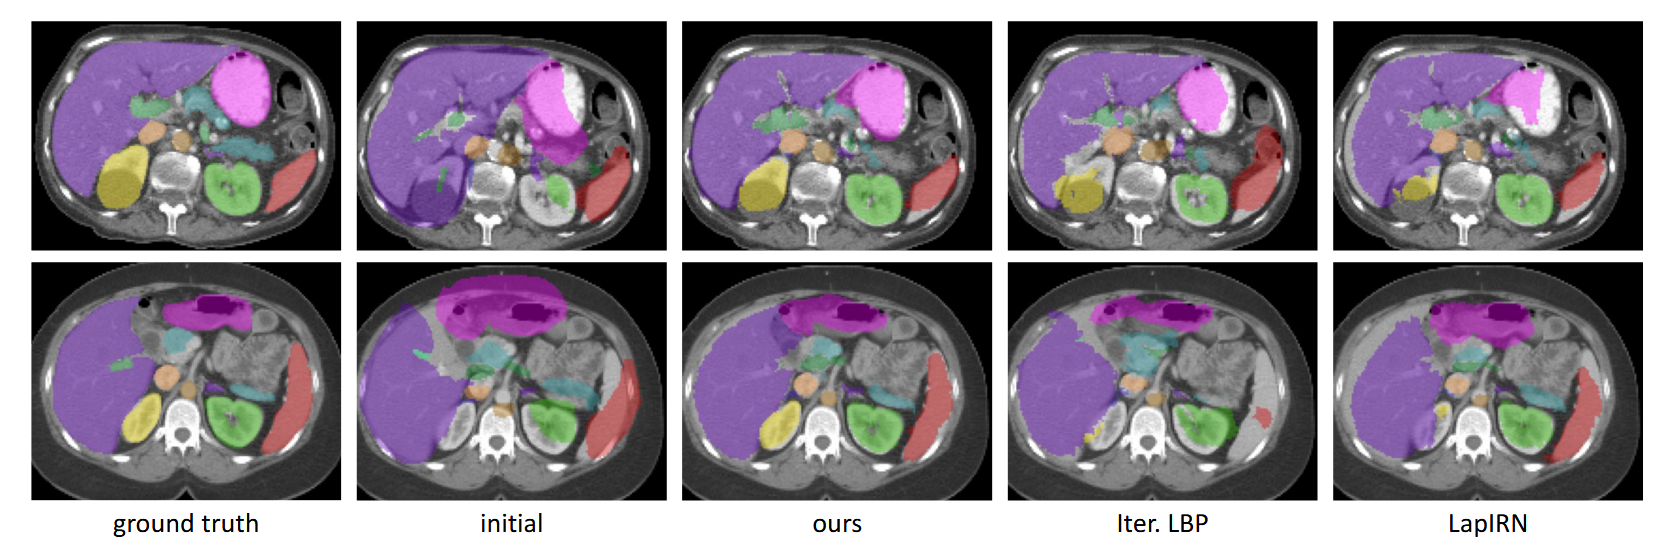
\includegraphics[width=0.9\textwidth]{T_img.png}
  \bicaption[t-fig:3]{}{所选方法对两例腹部CT数据集(轴向视图)的定性结果。我们展示了扭曲分割标签与固定扫描的叠加}{Fig.$\!$ }{Qualitative results of selected methods on two cases of the Abdomen CT dataset (axial view). We show overlays of the warped segmentation labels with the fixed scan.}
\end{figure}

\begin{table}
  \bicaption[t:table2]{}{无监督腹部CT配准结果}{Table$\!$}{Results for unsupervised abdomen CT registration.}
  \vspace{0.5em}\centering\wuhao
  \begin{tabular}{lccc}
    \toprule
    \textbf{Method} & \textbf{Dice [\%]} & \textbf{SDlogJ} & \textbf{Time [s]} \\
    \midrule
    pre-aligned     & 25.9               & --              & --                \\
    Adam            & 36.6               & 0.080           & 1.6               \\
    Iter. LBP       & 40.1               & 0.093           & 0.6               \\
    ANTs (SyN)      & 28.4               & {N/A}           & 74.3              \\
    DEEDS           & 46.5               & {N/A}           & 45.4              \\
    \midrule
    VoxelMorph      & 35.4               & 0.134           & 0.2               \\
    PDD             & 41.5               & 0.129           & 1.4               \\
    LapIRN          & 42.4               & 0.089           & 3.8               \\
    SAME            & 49.8               & {N/A}           & 1.2               \\
    \midrule
    MIND sup.       & 47.7               & 0.237           & 1.2               \\
    NCC sup.        & 48.1               & 0.299           & 1.2               \\
    \midrule
    ours            & \textbf{51.1}      & 0.146           & 1.2               \\
    \bottomrule
  \end{tabular}
\end{table}

\textbf{Lung. }For point cloud-based lung registration, we compare our cyclical selftraining strategy to three alternative learning strategies: supervision with manually annotated landmark correspondences as in [9], metric-based supervision with Chamfer distance and local Laplacian penalties as in [23], and training on synthetic rigid/random field deformations. All strategies are implemented for the same baseline registration model from [9]. Moreover, we report the performance of three unsupervised image-based deep learning methods [2,12,17] trained with MIND supervision. Results are shown in Tab.3, demonstrating the superiority of our self-training strategy over all competing learning strategies and the reported image-based SOTA methods. Qualitative results of the experiment are shown in Supp., Fig.4, demonstrating accurate and smooth displacements, as also confirmed by low values of SDlogJ.

\begin{table}
  \bicaption[t:table3]{}{COPD数据集上的肺部CT配准结果}{Table$\!$}{Results for lung CT registration on the COPD dataset.}
  \vspace{0.5em}\centering\wuhao
  \begin{tabular}{lcc}
    \toprule
    \textbf{Method}       & \textbf{TRE [mm]} & \textbf{SDlogJ} \\
    \midrule
    initial (pre-aligned) & 11.99             & --              \\
    VoxelMorph            & 7.98              & {N/A}           \\
    LapIRN                & 4.99              & {N/A}           \\
    PDD                   & 2.16              & {N/A}           \\
    \midrule
    rigid deform.         & 2.98              & 0.037           \\
    rnd. field deform.    & 3.19              & 0.035           \\
    metric sup.           & 6.79              & 0.042           \\
    landmark sup.         & 2.27              & 0.036           \\
    \midrule
    ours                  & \textbf{1.93}     & 0.033           \\
    \bottomrule
  \end{tabular}
\end{table}

\section{Conclusion}

We introduced a novel cyclical self-training paradigm for unsupervised registration. To this end, we developed a modular registration pipeline of a deep feature extraction network coupled with a differentiable optimizer, stabilizing learning from noisy pseudo labels through regularization and iterative, cyclical refinement. That way, our method avoids pitfalls of popular metric supervision (NCC, MIND), which relies on shallow features or image intensities and is prone to noise and local minima. By contrast, our supervision through optimization-refined and -regularized pseudo labels promotes learning task-specific features that are more robust to noise, and our cyclical learning strategy gradually improves the expressiveness of features to avoid local minima. In our experiments, we demonstrated the efficacy and flexibility of our approach, which outperformed the competing state-of-the-art methods and learning strategies for dense image-based abdomen and point cloud-based lung registration. In summary, we did not only present the first fully unsupervised self-training scheme but also a new perspective on unsupervised learning-based registration. In particular, we consider our strategy complementary to existing techniques (metric-based and contrastive learning), opening up the potential for combined training schemes in future work.



\chapter{外文资料翻译}
\label{cha:chorg}
\title{基于优化引导循环自训练的无监督三维配准方法}
\textbf{摘要:}当前最先进的深度学习配准方法采用三种学习策略:需要昂贵人工标注的监督学习、严重依赖领域专家设计的人工相似性度量的无监督学习,以及存在领域偏移问题的合成数据训练方法。为了克服这些策略的局限,我们提出了一种基于自训练机制的新型自监督学习范式。该方法基于两个关键洞见:1)基于特征的可微分优化器即使使用随机特征也能完成合理配准;2)该优化器能稳定特征提取网络在噪声标签下的训练。因此我们提出循环自训练框架:首先通过随机特征推导位移场初始化伪标签,随后基于特征提取网络生成的增强特征循环更新伪标签,最终形成自我强化效应。在腹部和肺部配准任务上的实验表明,本方法显著超越基于相似性度量的监督方法,性能优于多种当前最先进的对比方法。源码详见 https://github.com/multimodallearning/reg-cyclical-self-train。

\section{介绍}

医学图像配准是医学影像领域的基础任务,其应用涵盖多模态数据融合及时序数据分析等多个方面。近年来,深度学习推动了基于学习的配准方法发展[11],这些方法在保证较低运行时间的同时实现了具有竞争力的性能,成为传统优化方法(精度高但速度慢)的有力替代方案。成功训练深度学习模型的关键在于选择合适的训练监督策略。现有文献主要包含三种学习策略:第一种是基于人工标注(如关键点对应关系[9]或语义标签[16])的监督学习。然而人工标注成本高昂且可能引入标签偏差[2]。第二种策略利用合成形变场生成具有精确已知位移场的图像对[7],但这种方法会在合成训练数据与真实测试数据之间产生领域差异,导致推理阶段性能受限。虽然精细的形变生成技术可以缩小这种差异,但需要深厚的领域知识、面向特定问题定制,且缺乏跨任务的泛化能力。第三种广泛应用的无监督度量学习方法通过最大化固定图像与形变移动图像之间的相似性指标实现训练(如[2,17]的实现),常用指标包括归一化互相关[19]和MIND[13]等。但该策略的效果高度依赖于人工设计的特定指标,且训练得到的深度学习模型性能常逊色于基于优化的经典方法。针对上述训练技术的不足,本研究提出基于自训练概念的新型无监督配准学习策略。自训练是半监督学习[24]和领域自适应[29]中的常用策略,其核心思想是先基于标注数据预训练网络,随后应用该模型于未标注数据生成伪标签,最后通过标注数据与伪标签数据的联合训练与伪标签更新交替进行。该范式已在多种任务中成功应用,其中医学领域方法主要集中于分割任务[8,18],这类方法采用自训练的特殊形式——Mean Teacher范式[22],通过教师模型(学习网络的时序集成)持续提供伪标签。传统自训练方法与基于Mean Teacher的方法均面临伪标签固有噪声的问题,这种噪声会严重影响学习过程。对此,部分研究尝试基于模型不确定性筛选可靠伪标签[28]。最近,Mean Teacher方法开始被应用于配准问题处理领域自适应[3]或补充基于度量的监督以实现自适应正则化加权[25]。与现有方法不同,本文首次将自训练引入完全无监督的配准场景,将伪标签作为唯一的监督来源。

\textbf{贡献.}
本文提出了一种适用于无监督配准任务的新型自训练学习范式,这一创新涉及两大核心挑战的解决。首先,在预训练阶段缺乏标注数据的情况下,如何生成初始伪标签成为关键问题。其次,需要有效缓解自训练过程中伪标签噪声的负面影响。通过将基于深度学习的特征提取与可微分优化算法(如[9,20])相结合进行位移预测研究,我们获得了两项重要发现(见图2)。首先,我们发现基于特征的优化器即使使用随机特征网络输出的特征(图2橙色曲线),仍能预测合理的位移场并改进初始配准结果。这归因于深度神经网络的归纳偏置特性——即使网络权重未经训练也能提取具有一定效用的特征[4]。这一特性使得预测位移场可成为有效的初始伪标签,从而解决首个挑战。针对第二个噪声标签问题,我们观察到优化器固有的正则化能力能够稳定噪声标签下的学习过程。具体而言,基于初始伪标签训练特征提取器所产生的配准精度(图2中绿、红、紫、棕及品红曲线)显著超越了训练所用噪声标签的精度水平。基于此,我们提出了循环自训练框架:通过特征提取器训练与伪标签更新的交替迭代,构建无需人工标注、避免合成形变领域偏移、且不依赖人工设计相似性度量的新型学习范式。与基于不确定性的伪标签过滤策略不同,本方法通过深度融合深度特征学习与正则化可微分优化,实现了噪声负面影响的隐式消除。通过在CT腹部配准及基于关键点的肺部配准任务上的实验验证,本方法相比多种最先进对比方案展现出显著性能提升。

\section{方法}

\subsection{问题定义}
给定固定图像$F$和移动图像$M$构成的数据对作为输入,配准任务旨在寻找将$M$与$F$空间对齐的位移场$\varphi$。我们在无监督设置下处理该任务,此时训练数据$\mathcal{T}=\{(\boldsymbol{F}_i,\boldsymbol{M}_i)\}_{i=1}^{|\mathcal{T}|}$包含$|\mathcal{T}|$个无标注数据对。基于训练数据,我们的目标是学习由参数$\theta_f$控制的函数$f$(部分通过深度网络实现),该函数可预测位移场$\hat{\boldsymbol{\varphi}}=f(\boldsymbol{F},\boldsymbol{M};\boldsymbol{\theta}_f)$。

\subsection{循环自训练}
为解决上述问题,我们提出如图1所示的循环自训练策略。传统自训练方法假设存在部分标注数据,但在无监督设置下这些标注不可得。为突破此限制并生成初始伪标签集用于自训练首阶段,我们将函数$f$参数化为两个组件的组合:1)用于特征提取的深度神经网络$g$;2)不可学习但可微分的基于特征优化算法$h$(用于位移预测),即:

\begin{figure}
  \centering
  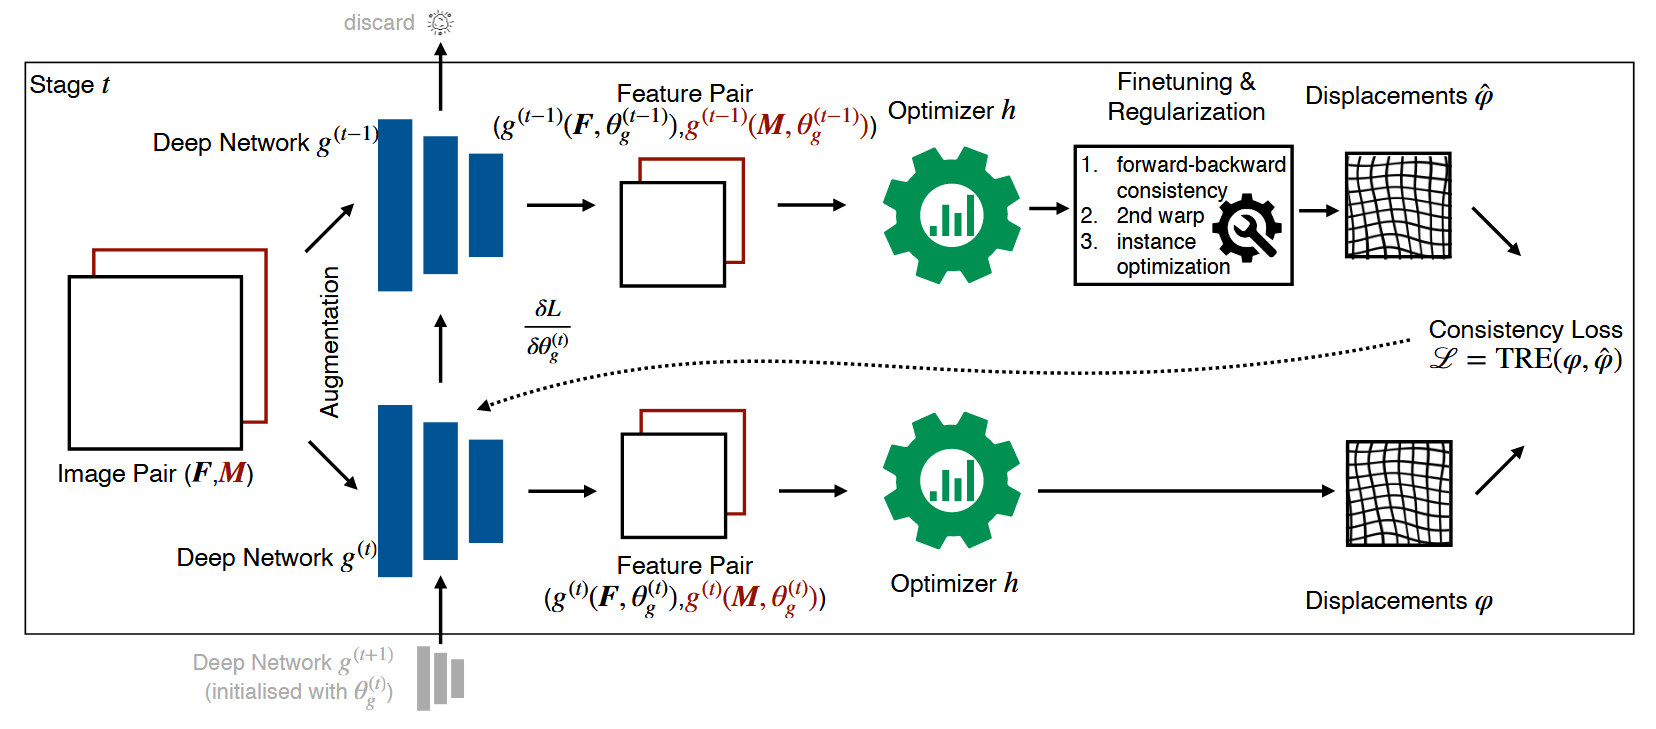
\includegraphics[width=0.9\textwidth]{T_RegCST.png}
  \bicaption[t-fig-c:1]{无监督注册的循环自训练范式概述}{底层配准流水线包括用于特征提取的深度网络g和用于预测位移的可微优化器h。在阶段t,我们使用基于前一阶段网络g(t-1)的特征生成的伪标签来监督网络g(t)的训练。对于最优特征学习,优化器的伪位移被进一步细化和正则化。}{Fig.$\!$ }{Overview of the proposed cyclical self-training paradigm for unsupervised registration. The underlying registration pipeline comprises a deep network for feature extraction g and a differentiable optimizer h to predict the displacements. At stage t, we supervise the training of the network $g^{(t)}$ with pseudo labels generated based on the features from the network $g^{(t-1)}$ from the previous stage. For optimal feature learning, the pseudo displacements from the optimizer are further refined and regularized.}
\end{figure}

\begin{equation}\tag*{(1)}
  f(\boldsymbol{F},\boldsymbol{M};\boldsymbol{\theta}_f)=h(g(\boldsymbol{F},\boldsymbol{M};\boldsymbol{\theta}_g))
\end{equation}

该方法基于我们的一项实证发现:即使使用随机初始化网络$g^{(0)}$(参数为$\theta_G^{(0)}$)提供的随机特征,合适的优化算法$h$仍能预测出合理的初始位移场$\hat{\boldsymbol{\varphi}}^{(0)}$,这与近期关于CNN归纳偏置的研究结论一致[4]。我们利用这些预测位移场作为伪标签来监督自训练的首阶段,通过最小化以下损失函数优化特征提取网络参数$\theta_G^{(1)}$:
\begin{equation}\tag*{(2)}
  \mathcal{L}(\boldsymbol{\theta}_g^{(1)};\mathcal{T})=\frac{1}{|\mathcal{T}|}\sum_i\mathrm{TRE}\left(h\left(g\left(\boldsymbol{F}_i,\boldsymbol{M}_i;\boldsymbol{\theta}_g^{(1)}\right)\right),\hat{\boldsymbol{\varphi}}_i^{(0)}\right)
\end{equation}
其中$\mathrm{TRE}(\hat{\boldsymbol{\varphi}}_\mathrm{i}^{(1)},\hat{\boldsymbol{\varphi}}_\mathrm{i}^{(0)})$表示位移场$\hat{\boldsymbol{\varphi}}_\mathrm{i}^{(1)}$与$\hat{\boldsymbol{\varphi}}_\mathrm{i}^{(0)}$逐元素目标配准误差的均值。

该基础框架存在网络可能过拟合初始伪标签并学习复制随机特征的关键问题。受对比学习最新技术启发[6],我们提出在学习和伪标签生成双路径中引入双重非对称性以增强特征学习效果:首先对双路径输入数据施加不同的随机增强;其次在伪标签路径的优化器后增加(不可微)细调与正则化步骤以提升伪位移场质量(详见第2.3节)。消融实验表明(图2、表1),这两种策略均可有效改善特征学习并强化自我增强效应。

当首阶段自训练收敛后,我们重复该过程$T$次迭代。具体而言,在第$t$阶段:1)使用前一阶段训练网络$g^{(t-1)}$生成精炼伪标签;2)以$g^{(t-1)}$权重初始化当前网络$g^{(t)}$;3)对学习率执行热重启以跳出前一阶段的局部极小值。

\subsection{配准框架}

我们提出的自训练方案是一个灵活、模块化的框架,其独立于输入模态及特征提取器$g$与优化器$h$的具体实现。本节阐述我们在图像和点云配准任务中对$g$和$h$的具体设计选择,其中图像配准为本文主要研究重点。

\textbf{图像配准.} 针对三维输入体数据,我们采用标准3D CNN实现特征提取器$g$。该网络包含六个卷积层,卷积核尺寸为3$\times$3$\times$3,通道数分别为32、64或128。每个卷积层后接批量归一化(BatchNorm)和ReLU激活函数,每隔一个卷积层进行步长为2的下采样,最终获得8倍降采样特征。通过1$\times$1$\times$1卷积将两幅图像特征映射至16维,并输入相关层[21]捕获125个离散位移。

作为优化器,我们基于文献[20]提出的耦合凸优化方法实现三维配准。该方法以固定和移动图像特征为输入,通过最小化平滑性与特征差异的联合目标函数推断位移场。伪标签流中的细化策略包含三个关键要素:1) 前向-后向一致性:额外计算反向位移场($\boldsymbol{F}$到$\boldsymbol{M}$),并通过迭代优化最小化双向场间差异;2) 二次形变:使用当前位移场对移动图像进行形变后重复前述步骤;3) 迭代实例优化:采用Adam算法联合最小化正则化代价与特征差异,对最终位移场进行微调。其中特征差异计算使用第二卷积块后的CNN特征(经1$\times$1$\times$1卷积映射至16通道)。在测试阶段采用相同的细化步骤。

此外,我们提出通过比较网络预测位移与微调后位移的差异来估计训练样本难度。据此实施加权批量采样策略,优先选择场间一致性更高的简单配准对。具体实现中,对所有训练对进行难度排序,并采用参数范围-5至5的sigmoid函数构建加权随机采样器。

\textbf{点云配准.} 对于点云配准任务,我们采用图卷积网络实现特征提取器,并基于文献[9]提出的可微分稀疏循环置信传播算法进行优化。

\section{实验}

\subsection{实验设置}

\textbf{数据集.} 我们在Learn2Reg (L2R)挑战赛[15]的跨患者腹部CT配准数据集上进行主要实验。该数据集包含30例不同患者的三维腹部CT扫描数据,包含13个尺寸差异显著的手动标注解剖结构。原始影像数据与标签来源于[26]。作为L2R基准的一部分,数据经仿射预配准至标准空间,并重采样为统一体素分辨率(2毫米)和空间维度(192$\times$160$\times$256体素)。遵循L2R数据划分方案,使用20例扫描(190对)进行训练,剩余10例(45对)用于评估。数据划分与预处理流程与对比方法[9,27]保持一致。评估指标采用语义标签间的平均Dice相似系数(DSC)及对数雅可比行列式标准差(SDlogJ)。

我们使用DIR-Lab COPDGene数据集[5]进行呼气-吸气相位肺部CT配准的补充实验,该数据集包含10组扫描对。每组扫描提供300个专家标注的解剖标志点用于评估。预处理流程包含:1) 呼气相扫描重采样至1.75$\times$1.00$\times$1.25毫米,吸气相至1.75$\times$1.25$\times$1.75毫米;2) 基于自动生成肺部分割掩膜,截取固定尺寸感兴趣区域(192$\times$192$\times$208体素);3) 对肺部分割结果进行仿射预配准。针对肺部CT关键点配准任务,我们遵循[9]的方法,使用Förstner算法结合非极大值抑制提取CT影像特征点,固定影像约生成1,000个点,移动影像约2,000个点。实验采用五折交叉验证,每折包含8对训练数据和2对测试数据。评估指标为标志点处目标配准误差(TRE)及SDlogJ。

\textbf{实现细节.} 所有方法基于PyTorch框架实现,使用Adam优化器进行网络参数优化。腹部配准任务设置$T$=8个训练阶段,每阶段包含1,000次迭代(batch size=2),学习率采用余弦退火热重启策略,每阶段从$10^{-3}$衰减至$10^{-5}$。超参数根据训练集三个病例的DSC指标确定。肺部配准任务经过$T$=5个阶段(每阶段60个epoch,batch size=4)达到收敛,初始学习率0.001,分别在第40和52 epoch衰减10倍。该任务超参数继承自[9]。两个数据集训练过程均在RTX2080显卡(8GB显存)上完成,耗时约90-100分钟,数据增强采用随机仿射变换。

\subsection{结果}

\textbf{腹部实验.} 首先通过消融实验分析本方法性能。图2展示了多个自训练周期中不同解剖结构类别的配准效果演变,可见各阶段性能持续提升(尤其在早期阶段显著),最终趋于收敛。这验证了伪标签更新与网络训练交替机制产生的自我增强效应。表1上半部分验证了双路径非对称增强(输入增强、伪标签微调)及加权采样策略的有效性,结果表明各组件对实现最优性能均具有重要作用。表1下半部分评估了不同测试配置下的模型表现,结果显示二次形变与Adam微调可带来显著性能提升。

\begin{figure}
  \centering
  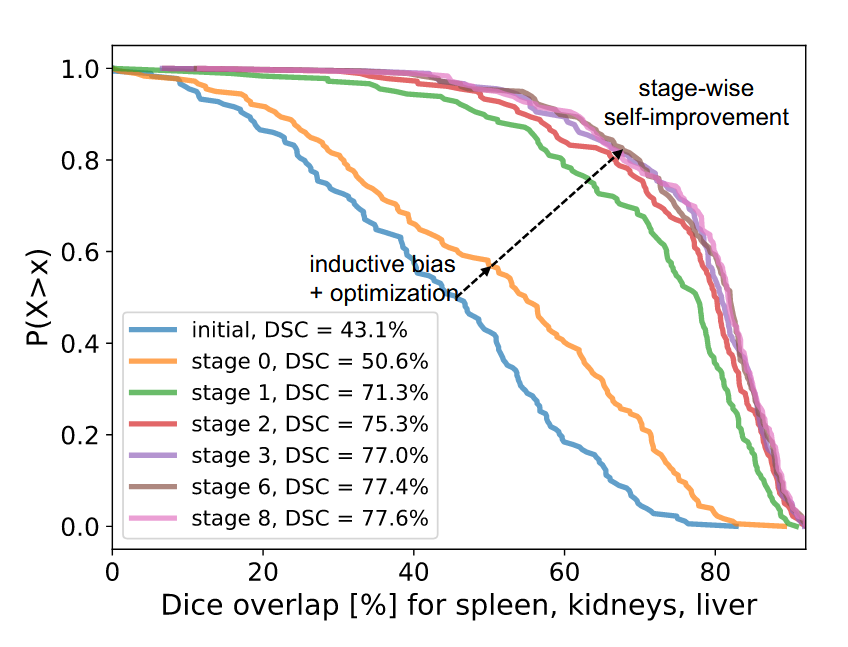
\includegraphics[width=0.9\textwidth]{T_result.png}
  \bicaption[t-fig-c:2]{}{在不同阶段的自我训练后,腹部CT登记的Dice重叠的“相反”累积分布。}{Fig.$\!$ }{“Opposite” cumulative distribution of Dice overlaps for Abdomen CT registration after different stages of self-training.}
\end{figure}

\begin{table}
  \bicaption[t-c:table1]{}{腹部CT配准的消融研究。}{Table$\!$}{Ablation study for abdomen CT registration.}
  \vspace{0.5em}\centering\wuhao
  \begin{tabular}{lcc}
    \toprule
    \textbf{Method}       & \textbf{DSC}  & \textbf{SDlogJ} \\
    \midrule
    prealign              & 25.9          & --              \\
    w/o input augm.       & 48.8          & 0.129           \\
    w/o PL refinement     & 48.8          & 0.200           \\
    w/o weighted sampling & 50.1          & 0.147           \\
    ours                  & 51.1          & 0.146           \\
    \midrule
    1 warp w/o Adam       & 38.6          & 0.061           \\
    1 warp w/ Adam        & 49.6          & 0.119           \\
    2 warps w/o Adam      & 41.1          & 0.088           \\
    2 warps w/Adam (ours) & \textbf{51.1} & 0.146           \\
    \bottomrule
  \end{tabular}
\end{table}

随后,我们将本方法与包括经典算法[1,10,14]和深度学习方法在内的多种最先进无监督方法进行对比,其中深度学习方法涵盖MIND[2,12]/NCC[17]监督训练和对比学习[27]方案。对比数据引自文献[9]与[27]。为直接验证自训练策略优势,我们还使用基于度量的监督方法(MIND[13]、NCC[19])训练了相同框架。实验结果见表2、图3及补充材料图3。本方法在DSC指标上显著超越所有对比方法(对公开代码方法进行Wilcoxon符号秩检验,p<0.0001;SAME方法因未公开代码未参与检验),以51.1\%的DSC刷新当前最佳性能。这证明了新学习范式相较于传统无监督策略的优越性。同时,预测位移场的平滑性指标(SDlogJ)与多数无监督深度方法[2,12]相当,且优于MIND与NCC监督方法。

\begin{figure}
  \centering
  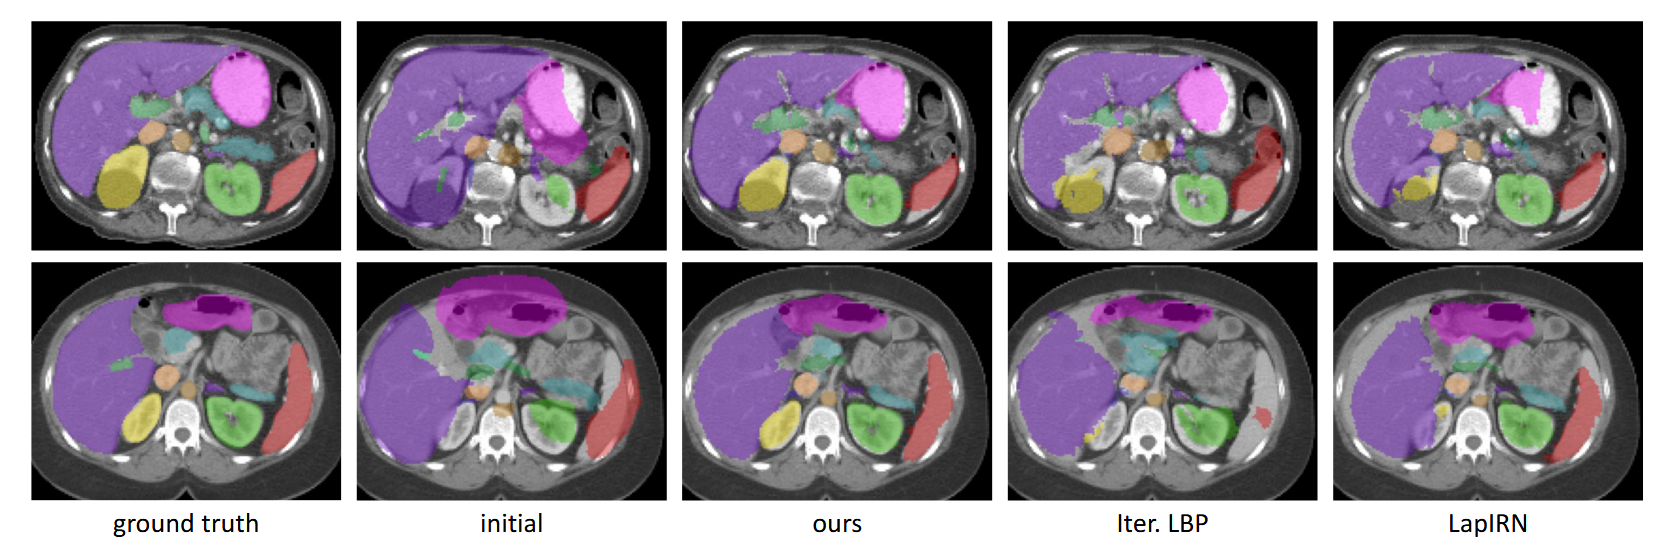
\includegraphics[width=0.9\textwidth]{T_img.png}
  \bicaption[ct-fig:3]{}{所选方法对两例腹部CT数据集(轴向视图)的定性结果。我们展示了扭曲分割标签与固定扫描的叠加}{Fig.$\!$ }{Qualitative results of selected methods on two cases of the Abdomen CT dataset (axial view). We show overlays of the warped segmentation labels with the fixed scan.}
\end{figure}

\begin{table}
  \bicaption[ct:table2]{}{无监督腹部CT配准结果}{Table$\!$}{Results for unsupervised abdomen CT registration.}
  \vspace{0.5em}\centering\wuhao
  \begin{tabular}{lccc}
    \toprule
    \textbf{Method} & \textbf{Dice [\%]} & \textbf{SDlogJ} & \textbf{Time [s]} \\
    \midrule
    pre-aligned     & 25.9               & --              & --                \\
    Adam            & 36.6               & 0.080           & 1.6               \\
    Iter. LBP       & 40.1               & 0.093           & 0.6               \\
    ANTs (SyN)      & 28.4               & {N/A}           & 74.3              \\
    DEEDS           & 46.5               & {N/A}           & 45.4              \\
    \midrule
    VoxelMorph      & 35.4               & 0.134           & 0.2               \\
    PDD             & 41.5               & 0.129           & 1.4               \\
    LapIRN          & 42.4               & 0.089           & 3.8               \\
    SAME            & 49.8               & {N/A}           & 1.2               \\
    \midrule
    MIND sup.       & 47.7               & 0.237           & 1.2               \\
    NCC sup.        & 48.1               & 0.299           & 1.2               \\
    \midrule
    ours            & \textbf{51.1}      & 0.146           & 1.2               \\
    \bottomrule
  \end{tabular}
\end{table}

\textbf{肺部实验.} 在基于点云的肺部配准任务中,我们将循环自训练策略与三种学习方案进行对比:1) 基于人工标注标志点的监督学习[9];2) 结合倒角距离与局部拉普拉斯惩罚的度量监督[23];3) 合成刚性/随机形变场训练。所有策略均基于文献[9]的基准模型实现。此外,我们还对比了三种基于MIND监督的无监督图像配准方法[2,12,17]。表3结果显示,本自训练策略在所有对比方案及现有图像配准SOTA方法中均表现出最优性能。补充材料图4展示了实验的定性结果,可见预测位移场兼具高精度与平滑性,该结论亦得到低SDlogJ值的支持。

\section{结论}

我们提出了一种新型的循环自训练范式用于无监督配准任务。为此,我们开发了模块化的配准流程框架,该框架将深度特征提取网络与可微分优化器相结合,通过正则化与迭代式循环精炼机制,有效稳定了噪声伪标签下的学习过程。相较于依赖浅层特征或图像强度的传统度量监督方法(如NCC、MIND)——这类方法易受噪声干扰并陷入局部极小——我们的优化驱动伪标签监督机制具有显著优势:1)基于优化精炼与正则化的伪标签能够引导网络学习更具噪声鲁棒性的任务相关特征;2)循环学习策略通过渐进式特征增强有效避免局部极小。实验结果表明,本方法在密集图像腹部配准与点云肺部配准任务中均超越当前最先进方法,充分验证了方案的有效性与灵活性。综上所述,本研究不仅首次实现了完全无监督的自训练框架,更为基于学习的无监督配准提供了全新视角。特别值得指出的是,本策略与现有技术(度量监督与对比学习)具有互补性,为未来构建联合训练方案开辟了新可能。

% \title{The title of the English paper}

% \textbf{Abstract:} As one of the most widely used techniques in operations
% research, \emph{ mathematical programming} is defined as a means of maximizing a
% quantity known as \emph{bjective function}, subject to a set of constraints
% represented by equations and inequalities. Some known subtopics of mathematical
% programming are linear programming, nonlinear programming, multiobjective
% programming, goal programming, dynamic programming, and multilevel
% programming$^{[1]}$.

% It is impossible to cover in a single chapter every concept of mathematical
% programming. This chapter introduces only the basic concepts and techniques of
% mathematical programming such that readers gain an understanding of them
% throughout the book$^{[2,3]}$.


% \section{Single-Objective Programming}
% The general form of single-objective programming (SOP) is written
% as follows,
% \begin{equation}\tag*{(123)} % 如果附录中的公式不想让它出现在公式索引中,那就请
%                              % 用 \tag*{xxxx}
% \left\{\begin{array}{l}
% \max \,\,f(x)\\[0.1 cm]
% \mbox{subject to:} \\ [0.1 cm]
% \qquad g_j(x)\le 0,\quad j=1,2,\cdots,p
% \end{array}\right.
% \end{equation}
% which maximizes a real-valued function $f$ of
% $x=(x_1,x_2,\cdots,x_n)$ subject to a set of constraints.

% \newtheorem{mpdef}{Definition}[chapter]
% \begin{mpdef}
% In SOP, we call $x$ a decision vector, and
% $x_1,x_2,\cdots,x_n$ decision variables. The function
% $f$ is called the objective function. The set
% \begin{equation}\tag*{(456)} % 这里同理,其它不再一一指定。
% S=\left\{x\in\Re^n\bigm|g_j(x)\le 0,\,j=1,2,\cdots,p\right\}
% \end{equation}
% is called the feasible set. An element $x$ in $S$ is called a
% feasible solution.
% \end{mpdef}

% \newtheorem{mpdefop}[mpdef]{Definition}
% \begin{mpdefop}
% A feasible solution $x^*$ is called the optimal
% solution of SOP if and only if
% \begin{equation}
% f(x^*)\ge f(x)
% \end{equation}
% for any feasible solution $x$.
% \end{mpdefop}

% One of the outstanding contributions to mathematical programming was known as
% the Kuhn-Tucker conditions\ref{eq:ktc}. In order to introduce them, let us give
% some definitions. An inequality constraint $g_j(x)\le 0$ is said to be active at
% a point $x^*$ if $g_j(x^*)=0$. A point $x^*$ satisfying $g_j(x^*)\le 0$ is said
% to be regular if the gradient vectors $\nabla g_j(x)$ of all active constraints
% are linearly independent.

% Let $x^*$ be a regular point of the constraints of SOP and assume that all the
% functions $f(x)$ and $g_j(x),j=1,2,\cdots,p$ are differentiable. If $x^*$ is a
% local optimal solution, then there exist Lagrange multipliers
% $\lambda_j,j=1,2,\cdots,p$ such that the following Kuhn-Tucker conditions hold,
% \begin{equation}
% \label{eq:ktc}
% \left\{\begin{array}{l}
%     \nabla f(x^*)-\sum\limits_{j=1}^p\lambda_j\nabla g_j(x^*)=0\\[0.3cm]
%     \lambda_jg_j(x^*)=0,\quad j=1,2,\cdots,p\\[0.2cm]
%     \lambda_j\ge 0,\quad j=1,2,\cdots,p.
% \end{array}\right.
% \end{equation}
% If all the functions $f(x)$ and $g_j(x),j=1,2,\cdots,p$ are convex and
% differentiable, and the point $x^*$ satisfies the Kuhn-Tucker conditions
% (\ref{eq:ktc}), then it has been proved that the point $x^*$ is a global optimal
% solution of SOP.

% \subsection{Linear Programming}
% \label{sec:lp}

% If the functions $f(x),g_j(x),j=1,2,\cdots,p$ are all linear, then SOP is called
% a {\em linear programming}.

% The feasible set of linear is always convex. A point $x$ is called an extreme
% point of convex set $S$ if $x\in S$ and $x$ cannot be expressed as a convex
% combination of two points in $S$. It has been shown that the optimal solution to
% linear programming corresponds to an extreme point of its feasible set provided
% that the feasible set $S$ is bounded. This fact is the basis of the {\em simplex
%   algorithm} which was developed by Dantzig as a very efficient method for
% solving linear programming.
% \begin{table}[ht]
% \centering
%   \centering
%   \caption*{Table~1\hskip1em This is an example for manually numbered table, which
%     would not appear in the list of tables}
%   \label{tab:badtabular2}
%   \begin{tabular}[c]{|m{1.5cm}|c|c|c|c|c|c|}\hline
%     \multicolumn{2}{|c|}{Network Topology} & \# of nodes &
%     \multicolumn{3}{c|}{\# of clients} & Server \\\hline
%     GT-ITM & Waxman Transit-Stub & 600 &
%     \multirow{2}{2em}{2\%}&
%     \multirow{2}{2em}{10\%}&
%     \multirow{2}{2em}{50\%}&
%     \multirow{2}{1.2in}{Max. Connectivity}\\\cline{1-3}
%     \multicolumn{2}{|c|}{Inet-2.1} & 6000 & & & &\\\hline
%     & \multicolumn{2}{c|}{ABCDEF} &\multicolumn{4}{c|}{} \\\hline
% \end{tabular}
% \end{table}

% Roughly speaking, the simplex algorithm examines only the extreme points of the
% feasible set, rather than all feasible points. At first, the simplex algorithm
% selects an extreme point as the initial point. The successive extreme point is
% selected so as to improve the objective function value. The procedure is
% repeated until no improvement in objective function value can be made. The last
% extreme point is the optimal solution.

% \subsection{Nonlinear Programming}

% If at least one of the functions $f(x),g_j(x),j=1,2,\cdots,p$ is nonlinear, then
% SOP is called a {\em nonlinear programming}.

% A large number of classical optimization methods have been developed to treat
% special-structural nonlinear programming based on the mathematical theory
% concerned with analyzing the structure of problems.

% Now we consider a nonlinear programming which is confronted solely with
% maximizing a real-valued function with domain $\Re^n$.  Whether derivatives are
% available or not, the usual strategy is first to select a point in $\Re^n$ which
% is thought to be the most likely place where the maximum exists. If there is no
% information available on which to base such a selection, a point is chosen at
% random. From this first point an attempt is made to construct a sequence of
% points, each of which yields an improved objective function value over its
% predecessor. The next point to be added to the sequence is chosen by analyzing
% the behavior of the function at the previous points. This construction continues
% until some termination criterion is met. Methods based upon this strategy are
% called {\em ascent methods}, which can be classified as {\em direct methods},
% {\em gradient methods}, and {\em Hessian methods} according to the information
% about the behavior of objective function $f$. Direct methods require only that
% the function can be evaluated at each point. Gradient methods require the
% evaluation of first derivatives of $f$. Hessian methods require the evaluation
% of second derivatives. In fact, there is no superior method for all
% problems. The efficiency of a method is very much dependent upon the objective
% function.

% \subsection{Integer Programming}

% {\em Integer programming} is a special mathematical programming in which all of
% the variables are assumed to be only integer values. When there are not only
% integer variables but also conventional continuous variables, we call it {\em
%   mixed integer programming}. If all the variables are assumed either 0 or 1,
% then the problem is termed a {\em zero-one programming}. Although integer
% programming can be solved by an {\em exhaustive enumeration} theoretically, it
% is impractical to solve realistically sized integer programming problems. The
% most successful algorithm so far found to solve integer programming is called
% the {\em branch-and-bound enumeration} developed by Balas (1965) and Dakin
% (1965). The other technique to integer programming is the {\em cutting plane
%   method} developed by Gomory (1959).

% \hfill\textit{Uncertain Programming\/}\quad(\textsl{BaoDing Liu, 2006.2})

% \section*{References}
% \noindent{\itshape NOTE: These references are only for demonstration. They are
%   not real citations in the original text.}

% \begin{translationbib}
% \item Donald E. Knuth. The \TeX book. Addison-Wesley, 1984. ISBN: 0-201-13448-9
% \item Paul W. Abrahams, Karl Berry and Kathryn A. Hargreaves. \TeX\ for the
%   Impatient. Addison-Wesley, 1990. ISBN: 0-201-51375-7
% \item David Salomon. The advanced \TeX book.  New York : Springer, 1995. ISBN:0-387-94556-3
% \end{translationbib}

% \chapter{外文资料的调研阅读报告或书面翻译}

% \title{英文资料的中文标题}

% {\heiti 摘要:} 本章为外文资料翻译内容。如果有摘要可以直接写上来,这部分好像没有
% 明确的规定。

% \section{单目标规划}
% 北冥有鱼,其名为鲲。鲲之大,不知其几千里也。化而为鸟,其名为鹏。鹏之背,不知其几
% 千里也。怒而飞,其翼若垂天之云。是鸟也,海运则将徙于南冥。南冥者,天池也。
% \begin{equation}\tag*{(123)}
%  p(y|\mathbf{x}) = \frac{p(\mathbf{x},y)}{p(\mathbf{x})}=
% \frac{p(\mathbf{x}|y)p(y)}{p(\mathbf{x})}
% \end{equation}

% 吾生也有涯,而知也无涯。以有涯随无涯,殆已!已而为知者,殆而已矣!为善无近名,为
% 恶无近刑,缘督以为经,可以保身,可以全生,可以养亲,可以尽年。

% \subsection{线性规划}
% 庖丁为文惠君解牛,手之所触,肩之所倚,足之所履,膝之所倚,砉然响然,奏刀騞然,莫
% 不中音,合于桑林之舞,乃中经首之会。
% \begin{table}[ht]
% \centering
%   \centering
%   \caption*{表~1\hskip1em 这是手动编号但不出现在索引中的一个表格例子}
%   \label{tab:badtabular3}
%   \begin{tabular}[c]{|m{1.5cm}|c|c|c|c|c|c|}\hline
%     \multicolumn{2}{|c|}{Network Topology} & \# of nodes &
%     \multicolumn{3}{c|}{\# of clients} & Server \\\hline
%     GT-ITM & Waxman Transit-Stub & 600 &
%     \multirow{2}{2em}{2\%}&
%     \multirow{2}{2em}{10\%}&
%     \multirow{2}{2em}{50\%}&
%     \multirow{2}{1.2in}{Max. Connectivity}\\\cline{1-3}
%     \multicolumn{2}{|c|}{Inet-2.1} & 6000 & & & &\\\hline
%     & \multicolumn{2}{c|}{ABCDEF} &\multicolumn{4}{c|}{} \\\hline
% \end{tabular}
% \end{table}

% 文惠君曰:“嘻,善哉!技盖至此乎?”庖丁释刀对曰:“臣之所好者道也,进乎技矣。始臣之
% 解牛之时,所见无非全牛者;三年之后,未尝见全牛也;方今之时,臣以神遇而不以目视,
% 官知止而神欲行。依乎天理,批大郤,导大窾,因其固然。技经肯綮之未尝,而况大坬乎!
% 良庖岁更刀,割也;族庖月更刀,折也;今臣之刀十九年矣,所解数千牛矣,而刀刃若新发
% 于硎。彼节者有间而刀刃者无厚,以无厚入有间,恢恢乎其于游刃必有余地矣。是以十九年
% 而刀刃若新发于硎。虽然,每至于族,吾见其难为,怵然为戒,视为止,行为迟,动刀甚微,
% 謋然已解,如土委地。提刀而立,为之而四顾,为之踌躇满志,善刀而藏之。”

% 文惠君曰:“善哉!吾闻庖丁之言,得养生焉。”


% \subsection{非线性规划}
% 孔子与柳下季为友,柳下季之弟名曰盗跖。盗跖从卒九千人,横行天下,侵暴诸侯。穴室枢
% 户,驱人牛马,取人妇女。贪得忘亲,不顾父母兄弟,不祭先祖。所过之邑,大国守城,小
% 国入保,万民苦之。孔子谓柳下季曰:“夫为人父者,必能诏其子;为人兄者,必能教其弟。
% 若父不能诏其子,兄不能教其弟,则无贵父子兄弟之亲矣。今先生,世之才士也,弟为盗
% 跖,为天下害,而弗能教也,丘窃为先生羞之。丘请为先生往说之。”

% 柳下季曰:“先生言为人父者必能诏其子,为人兄者必能教其弟,若子不听父之诏,弟不受
% 兄之教,虽今先生之辩,将奈之何哉?且跖之为人也,心如涌泉,意如飘风,强足以距敌,
% 辩足以饰非。顺其心则喜,逆其心则怒,易辱人以言。先生必无往。”

% 孔子不听,颜回为驭,子贡为右,往见盗跖。

% \subsection{整数规划}
% 盗跖乃方休卒徒大山之阳,脍人肝而餔之。孔子下车而前,见谒者曰:“鲁人孔丘,闻将军
% 高义,敬再拜谒者。”谒者入通。盗跖闻之大怒,目如明星,发上指冠,曰:“此夫鲁国之
% 巧伪人孔丘非邪?为我告之:尔作言造语,妄称文、武,冠枝木之冠,带死牛之胁,多辞缪
% 说,不耕而食,不织而衣,摇唇鼓舌,擅生是非,以迷天下之主,使天下学士不反其本,妄
% 作孝弟,而侥幸于封侯富贵者也。子之罪大极重,疾走归!不然,我将以子肝益昼餔之膳。”


% \chapter{其它附录}
% 前面两个附录主要是给本科生做例子。其它附录的内容可以放到这里,当然如果你愿意,可
% 以把这部分也放到独立的文件中,然后将其到主文件中。
